\begin{figure}[htb]
    \centering
    \caption{Correlation Between Median Rent Price (in dollars per square foot) and previous year change in MW (percentage).}
    \label{appfig:binsc_listing_mwpctchange}
    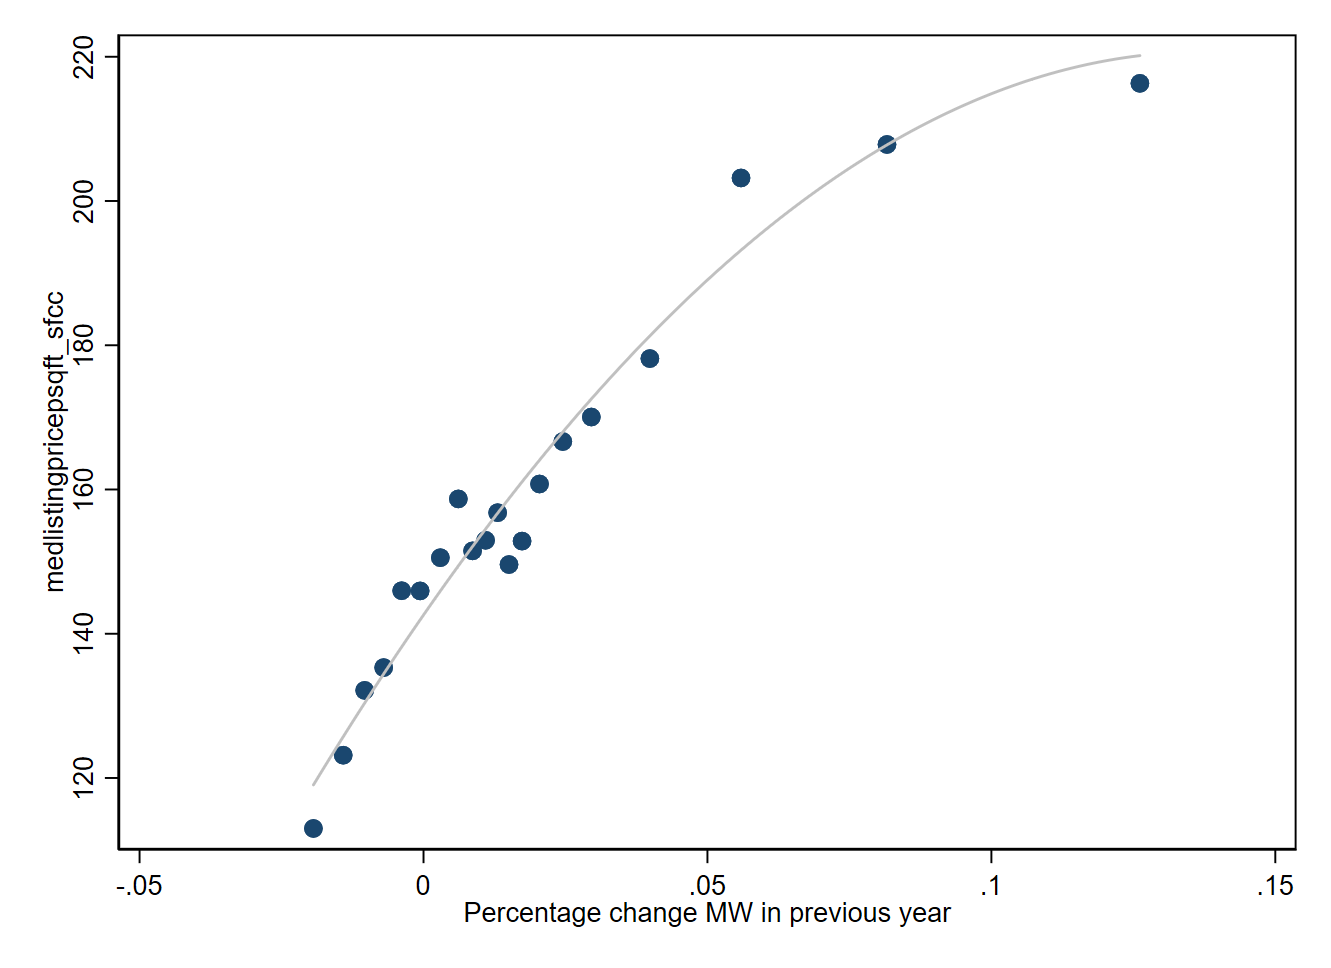
\includegraphics[width=0.75\linewidth]{draft_june20/tempfigure/binsc_medlistingpricepsqft_sfcc_pctMWch.png}
    \begin{minipage}{.95\textwidth} \footnotesize
		\vspace{2mm} 
		\textit{Notes}: The figure presents the correlation between median listing price on Zillow.com at the zipcode-year level and the percentage change in MW in the previous year. Data comes from the final sample used in the analysis (see \autoref{sec:data} for more details). Each zipcode yearly observation is obtained by averaging monthly observations, the basic time unit in this paper. The correlation is taken after controlling for year fixed effects, resident population, urban share, median income, black population share, and number of housing units.All demographic characteristics come from the 2010 Census.
	\end{minipage}
\end{figure}

\clearpage
\begin{figure}[htb] \centering
    \caption{Sensitivity of event study results to events selection - Main specification including control units}
    \label{appfig:event_size_sensitivity}
    \begin{subfigure}{0.5\textwidth} \centering
        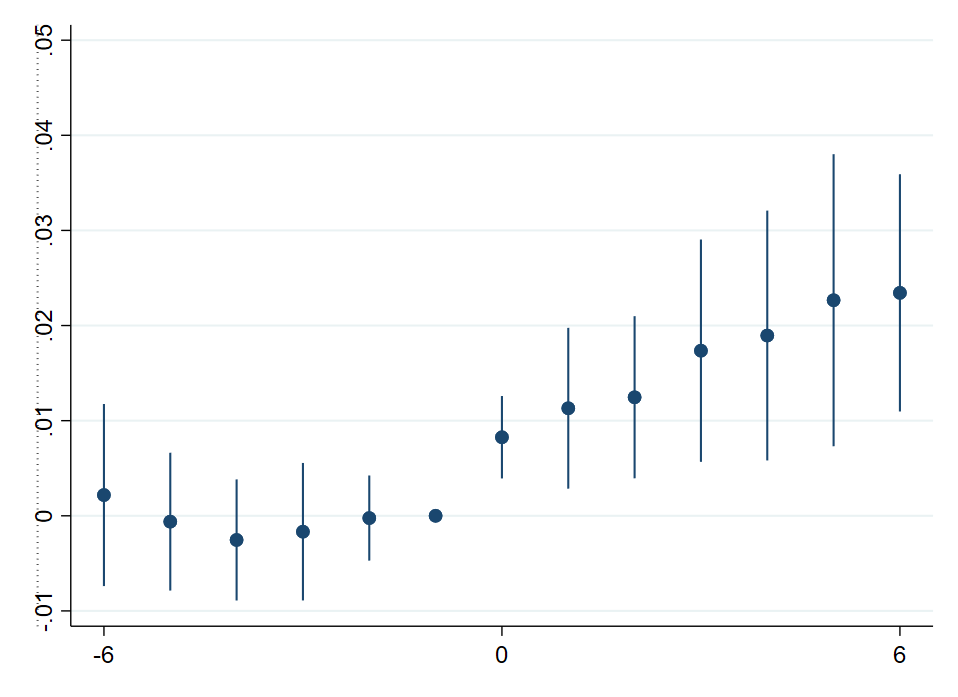
\includegraphics[width=0.95\linewidth]{analysis/event_size_robustness/output/last_rentpsqft_sfcc_event025_w6.png}
        \caption{Selecting events of at least \$0.25} \label{appfig:event_study_025_treated}
    \end{subfigure}%
    \begin{subfigure}{0.5\textwidth} \centering
        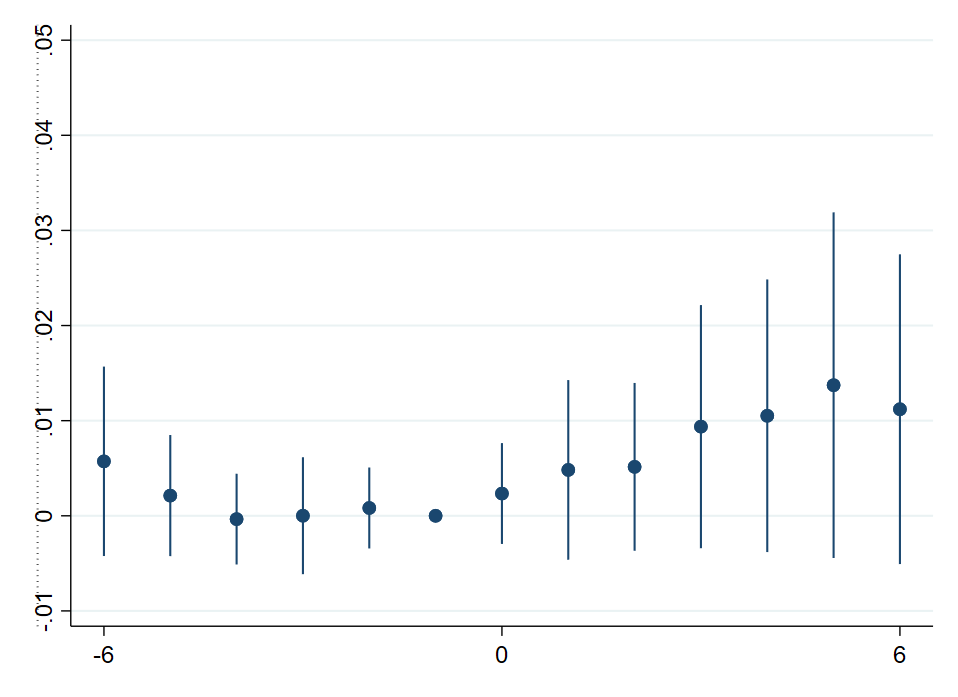
\includegraphics[width=0.95\linewidth]{analysis/event_size_robustness/output/last_rentpsqft_sfcc_event025_w6_county-trend.png}
        \caption{\begin{tabular}{c} Selecting events of at least \$0.25 \\ and county-specific trend \end{tabular}} \label{appfig:event_study_025_treated_county-trends}
    \end{subfigure}\\
    \begin{subfigure}{0.5\textwidth} \centering
        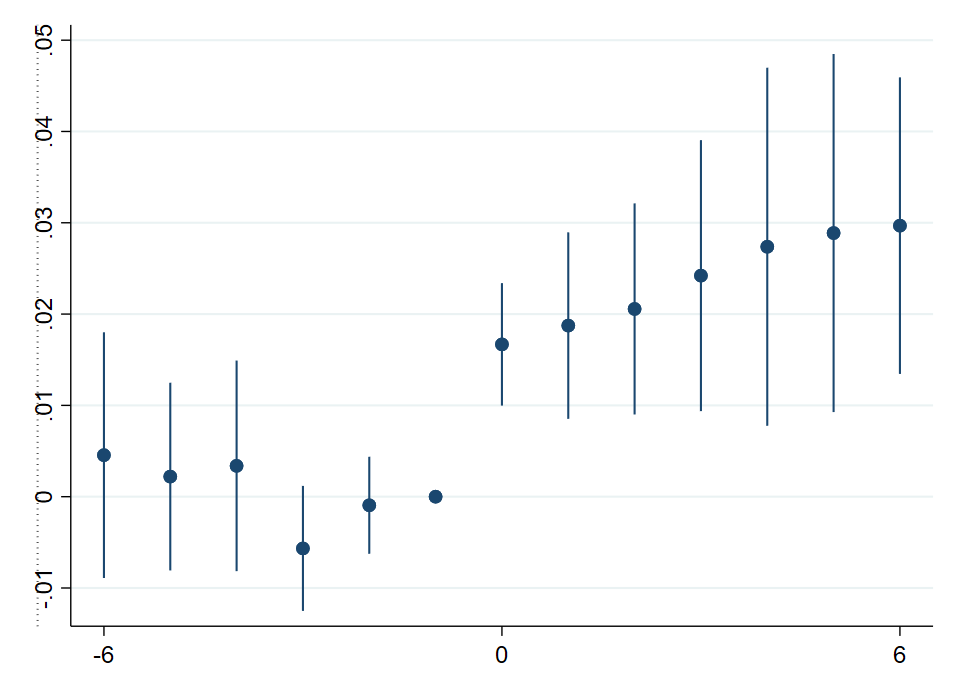
\includegraphics[width=0.95\linewidth]{analysis/event_size_robustness/output/last_rentpsqft_sfcc_event075_w6.png}
        \caption{Selecting events of at least \$0.75} \label{appfig:event_study_025_treated}
    \end{subfigure}%
    \begin{subfigure}{0.5\textwidth} \centering
        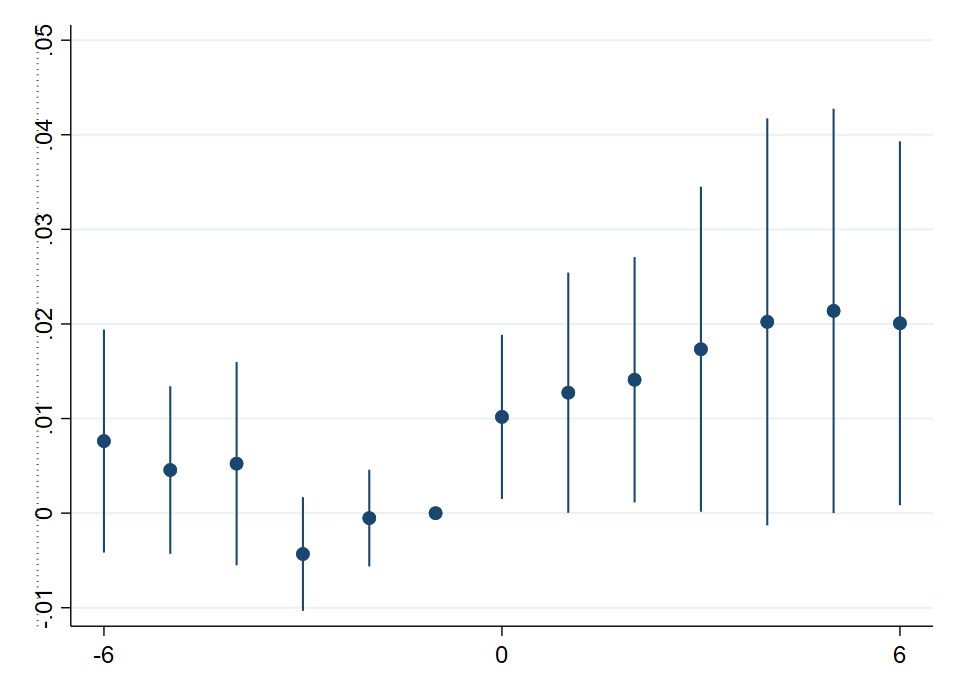
\includegraphics[width=0.95\linewidth]{analysis/event_size_robustness/output/last_rentpsqft_sfcc_event075_w6_county-trend.png}
        \caption{\begin{tabular}{c} Selecting events of at least \$0.75 \\ and county-specific trend \end{tabular}} \label{appfig:event_study_025_treated_county-trends}
    \end{subfigure}\\
    \begin{minipage}{.95\textwidth} \footnotesize
		\vspace{2mm} 
		\textit{Notes}: Results from fitting the ``last event'' event study with zipcode and calendar time fixed effects, controls for unused events, and including never treated zipcodes (esentially, this is the specification in the bottom row of \ref{fig:event_study_main}). All of the results select the last minimum wage event per zipcode, based on some cut-off and the requirement that it took place before June 2019 (so that every event has at least 6 months after it). The top row uses a cut-off of \$0.25, whereas the bottom row selects events based on a cut-off of \$0.75. Panels on the right add county-specific trends as controls.
	\end{minipage}
\end{figure}

\clearpage
\begin{figure}[htb] \centering
    \caption{Heterogeneity of effect - first difference model}
    \label{appfig:fd_heterogeneity_appendix}
    \begin{subfigure}{0.5\textwidth} \centering
        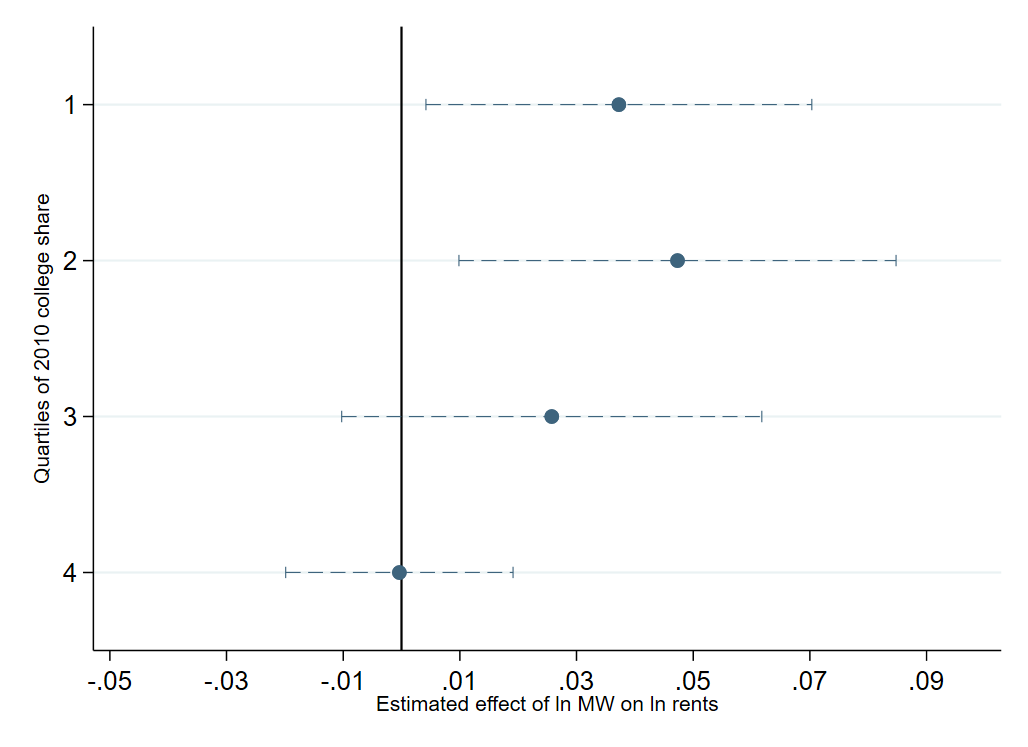
\includegraphics[width=0.99\linewidth]{analysis/first_differences/output/fd_static_heter_college_share20105.png}
        \caption{Share of college graduates in zipcode} \label{appfig:fd_heterogeneity_college_share}
    \end{subfigure}%
    \begin{subfigure}{0.5\textwidth} \centering
        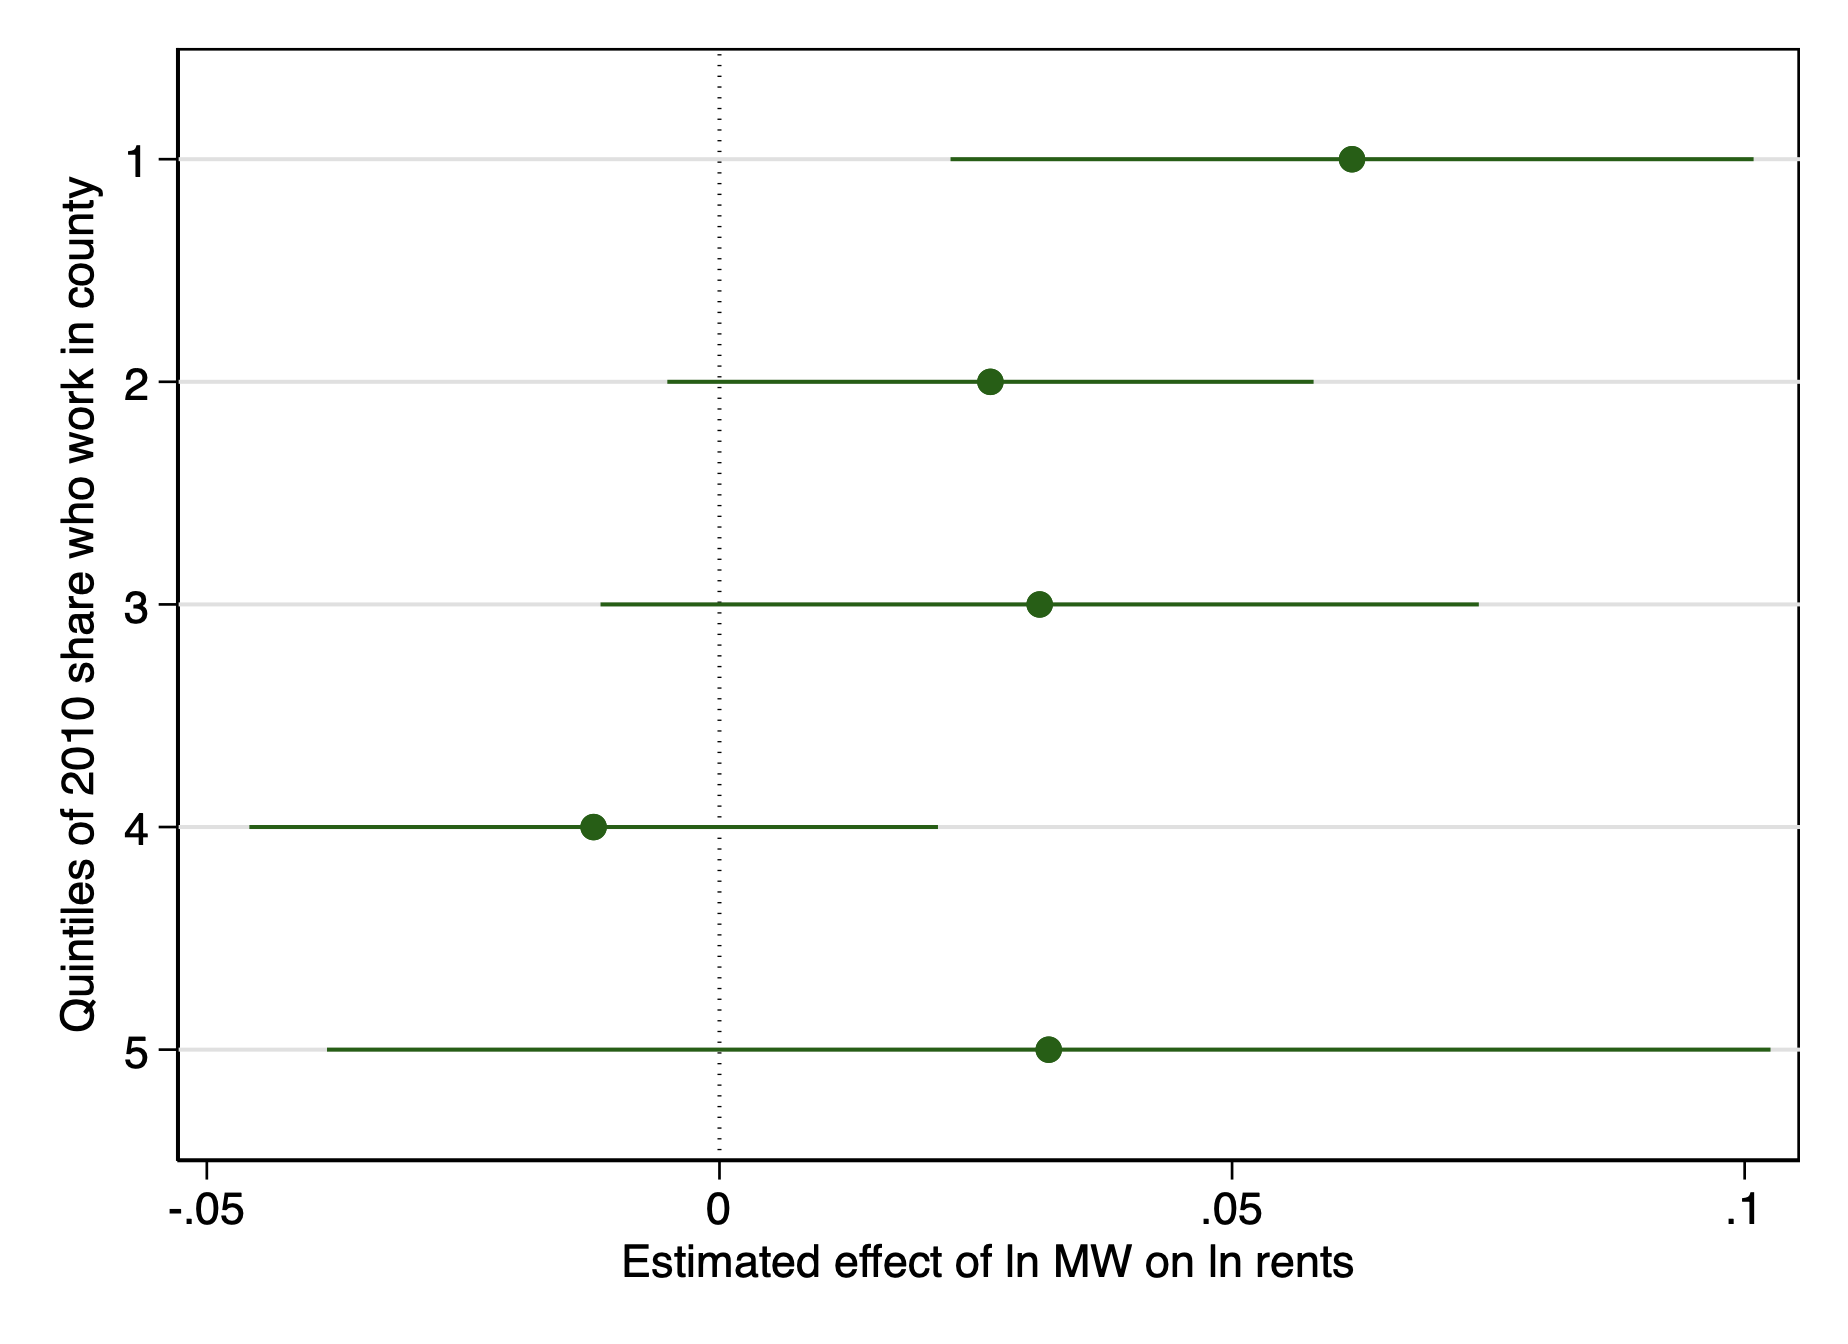
\includegraphics[width=0.99\linewidth]{analysis/first_differences/output/fd_static_heter_work_county_share20105.png}
        \caption{Share of individuals in zipcode who work in county} \label{appfig:fd_heterogeneity_work_county}
    \end{subfigure}\\
    \begin{subfigure}{0.5\textwidth} \centering
        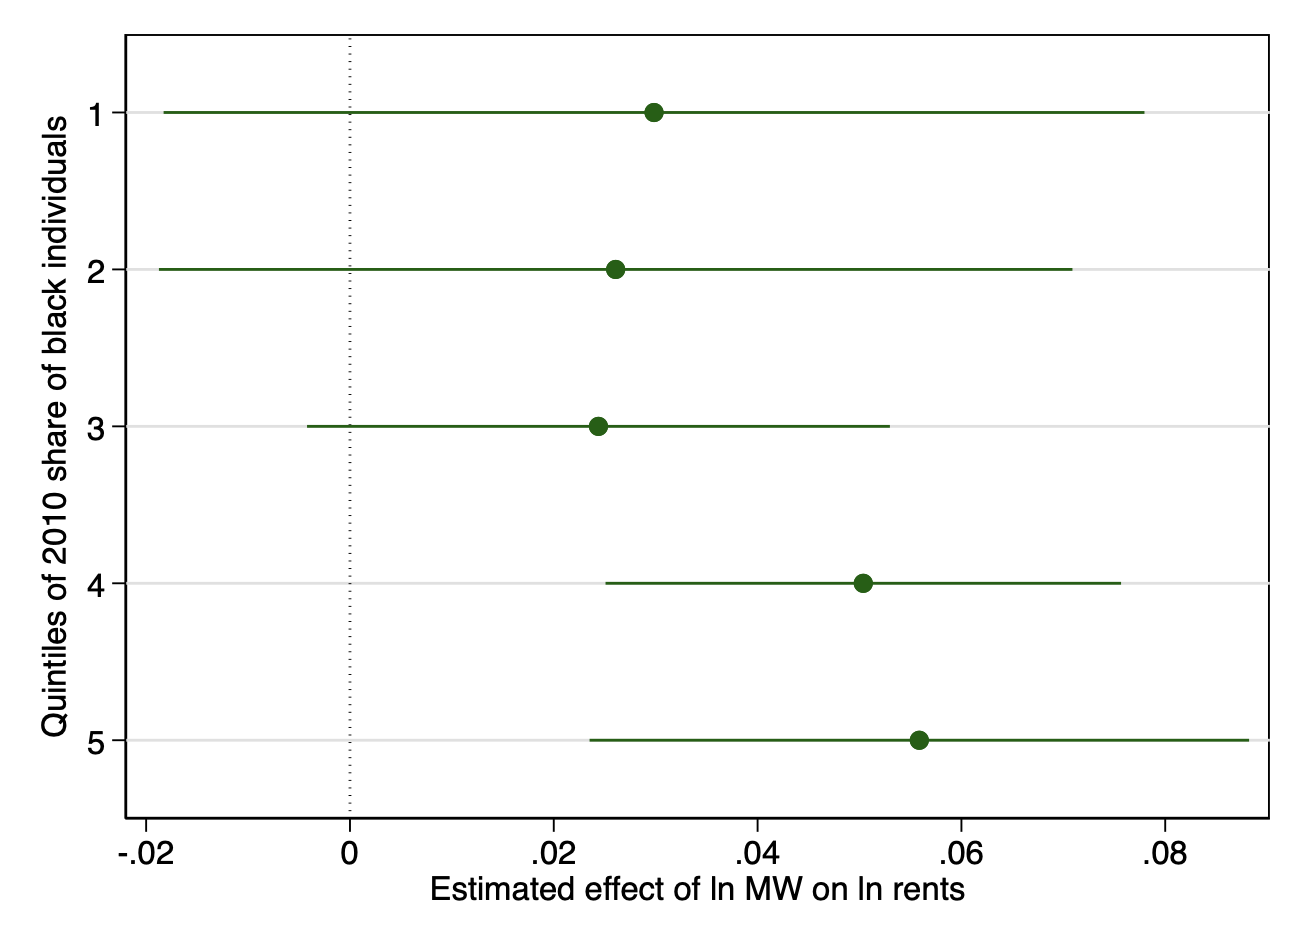
\includegraphics[width=0.99\linewidth]{analysis/first_differences/output/fd_static_heter_black_share2010.png}
        \caption{Share of black individuals} \label{appfig:fd_heterogeneity_work_county}
    \end{subfigure}\\
    \begin{minipage}{.95\textwidth} \footnotesize
		\vspace{2mm} 
		\textit{Notes}: The figure shows 
	\end{minipage}
\end{figure}
